\chapter{Evaluation}
\thispagestyle{fancy}
\label{chap:Evaluation}

\noindent
In diesem Kapitel werden alle Experimente umfangreich evaluiert. Dies geschieht einerseits auf Basis der ausgewählten Metriken, andererseits in Form einer qualitativen Analyse der aus den Anhängen A und B generierten Zusammenfassungen.


\section{Automatische Auswertung}
\noindent
In \autoref{table:ExpEvaluation} sind die \ac{ROUGE}-Scores der \ac{TF2TF} aller Experimente gesamtheitlich dokumentiert. Dabei werden die Experimente anhand der genutzten \ac{DLR} und der Sprache der eingegangenen Textdaten differenziert. Über die angefügte ID lassen sich die Experimente numerisch identifizieren und zuordnen.\\

\begin{table}[htb]
\centering
\begin{tabular}{ | p{1cm} | p{2.5cm} | p{2.5cm} | p{2.5cm} | p{2.5cm} | p{2.5cm} | }
\hline
\textbf{ID} & \textbf{DLR} & \textbf{Sprache} & \textbf{R-Recall} & \textbf{R-Precision} & \textbf{R-Measure} \\
\hline
1 & BERT & EN & 15.78 & 10.25 & 12.11 \\
\hline
1 & XLM-R & EN & 11.76 & 8.89 & 9.88 \\
\hline
2 & BERT & DE & 15.93 & 10.52 & 11.97 \\
\hline
2 & XLM-R & DE & 15.93 & 10.32 & 11.86 \\
\hline
3 & BERT & EN \& DE & 16.76 & 11.18 & 12.68 \\
\hline
3 & XLM-R & EN \& DE & 15.13 & 9.55 & 11.08 \\
\hline
3 & BART & EN \& DE & 19.39 & 11.08 & 13.73 \\
\hline
\end{tabular}
\caption{Ergebnisse im Experimentvergleich.}
\label{table:ExpEvaluation}
\end{table}

\noindent
Im ersten Experiment geschah die Reproduktion des \ac{SOTA} auf Basis englischsprachiger Daten. \ac{BERT} ist demnach unter Akzeptanz womöglich unbekannter Nebenbedingungen \ac{SOTA}-konform. \ac{XLM-R} hingegen bleibt weit zurück und bedarf aufgrund der komplexen Architektur einem noch umfangreicheren Fine-Tuning. Die Lernfortschritte sind anhand der Fehlerentwicklung in \autoref{pic:ExpEnLoss} visualisiert. Hierbei ist auch der Rückstand von \ac{XLM-R} nachvollziehbar.\\

\begin{figure}[h]
  \centering
  \fbox{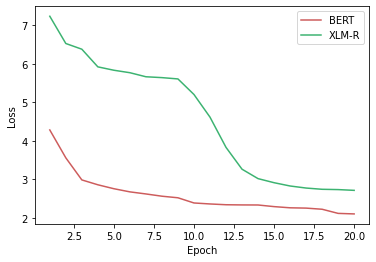
\includegraphics[width=0.6\linewidth]{./source/images/lossenglish.png}}
  \caption{Loss in der SOTA-Reproduktion im Modellvergleich.}
  \label{pic:ExpEnLoss}
\end{figure}

\noindent
Im zweiten Experiment geschah die Adaption der \ac{TF2TF} auf die deutsche Sprache. Hierfür kamen entsprechend ausschließlich deutschsprachige Daten zum Einsatz. \autoref{table:ExpEvaluation} gibt hierbei zu erkennen, dass \ac{BERT} wertmäßig in Englisch in etwa genauso gut wie in Deutsch ist. Der \ac{SOTA} wird indes unter Akzeptanz eines gewissen Rauschens von beiden Modellen erreicht. Die Lernfortschritte sind in bekannter Weise in \autoref{pic:ExpDeLoss} visualisiert. Hier ist zudem die Assimilation beider Modelle nachvollziehbar.\\

\begin{figure}[h]
  \centering
  \fbox{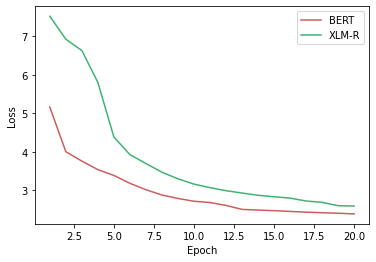
\includegraphics[width=0.6\linewidth]{./source/images/lossgerman.png}}
  \caption{Loss in der Adaption auf deutschen Daten im Modellvergleich.}
  \label{pic:ExpDeLoss}
\end{figure}
\newpage

\noindent
In dritten Experiment wurden alle verfügbaren Daten genutzt, um die \ac{TF2TF} einem Fine-Tuning zu unterziehen. \ac{BART} wird indes aus externer Quelle bezogen. In \autoref{table:ExpEvaluation} wird ersichtlich, dass sich \ac{BERT} unter multilingualen Trainingsdaten verbessert, \ac{XLM-R} hingegen nicht. \ac{BART} tritt wertmäßig deutlich hervor. In \autoref{pic:ExpMlLoss} wird zudem deutlich, dass \ac{XLM-R} erst spät, dann aber zielgerichtet trainiert. Hier scheint also die Nutzung umfangreicherer Trainingsdaten vielversprechend.\\

\begin{figure}[h]
  \centering
  \fbox{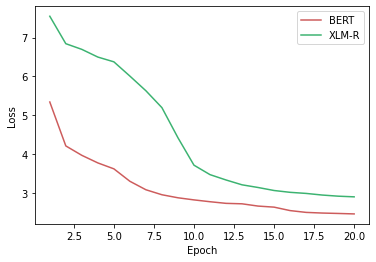
\includegraphics[width=0.6\linewidth]{./source/images/lossmultilingual.png}}
  \caption{Loss in der Adaption auf multilingualen Daten im Modellvergleich.}
  \label{pic:ExpMlLoss}
\end{figure}


\section{Qualitative Analyse}
\noindent
Die soeben evaluierten Experimente werden nun ergänzend qualitativ analysiert. Hierfür werden die \ac{TF2TF} aller Experimente sprachabhängig entweder Anhang A oder Anhang B unterzogen, indem die dort enthaltenen mitunter herausfordernden Texte maschinell zusammengefasst und subjektiv bewertet werden. Eine derartige Analyse ist erforderlich, um die Qualität sowie die praktische Eignung der trainierten \ac{TF2TF} vollends beurteilen zu können. Die qualitative Analyse ist außerdem erforderlich, um den teilweise kritisch begutachteten sowie eher statistisch veranlagten \ac{ROUGE}-Score qualitativ einzuordnen. Zudem sei bemerkt, dass die Zusammenfassungen in englischer und deutscher Sprache modellübergreifend den Anhängen C und D zu entnehmen sind.
\newpage

\noindent
Im ersten Experiment werden die englischen \ac{TF2TF} miteinander verglichen, namentlich \ac{BERT} und \ac{XLM-R}. Die obige Auswertung hebt hierbei \ac{BERT} als wertmäßig bestes Modell hervor. Die generierten Zusammenfassungen bestätigen diese Aussage aus praktischer Sicht für die getroffene Modellauswahl, obwohl Informationen teilweise leicht fehlerbehaftet sind. Dies wird im Kontext dieser Arbeit als \ac{SOTA}-konform interpretiert. \ac{XLM-R} hingegen ist unbrauchbar, insbesondere wegen der ungenügenden Grammatik und Orthographie. Somit sind auch viele der neu generierten Informationen schlichtweg falsch.\\

\noindent
Im zweiten Experiment werden die deutschen \ac{TF2TF} miteinander verglichen. Hier entspricht \ac{BERT} zwar wertmäßig dem \ac{SOTA}, schneidet jedoch vor allem bei Texten unbekannter Art eher schlecht ab. Dabei wird die Abhängigkeit des Modells von der Beschaffenheit der Trainingsdaten deutlich, insbesondere anhand der Natur der Zusammenfassungen. Hier ist nämlich ein typisches Element der Nachrichtendomäne erkennbar, da anstatt einer konventionellen Zusammenfassung oftmals ein Teaser generiert wird, der den Leser binden und zum Text weiterleiten soll. Dieses Verhalten ist jedoch nicht auf das Modell zurückzuführen, sondern auf die Trainingsdaten, welche größtenteils eben jener Nachrichtendomäne entstammen. Dies unterstreicht insgesamt die Notwendigkeit einer intensiven Datenanalyse. Hinsichtlich eines praktischen Einsatzes ist also stets ein anforderungsgerechter Korpus zu formieren. Zudem ist der Einfluss des vortrainierten Modells bemerkbar, beispielsweise im Text über das Finale der WM 2014. Hier wird im originalen Text von Jogi Löw geschrieben, in der Zusammenfassung hingegen von Jürgen Klopp. Letzterer wurde zuvor jedoch nie erwähnt. Dies kann mit der geringen Distanz beider Personen im Vektorraum erklärt werden und ist somit zwar sachlogisch falsch, mathematisch jedoch nachvollziehbar. Dies tritt in ähnlicher Weise auch in den anderen Zusammenfassungen auf. Ein Fine-Tuning mit sehr viel mehr Trainingsdaten verspricht dieses Rauschen hinreichend zu minimieren. Die deutsche \ac{XLM-R} lässt eine Verbesserung gegenüber der englischen \ac{XLM-R} vermuten. Dies lässt sich mithilfe der qualitativen Analyse bestätigen. Die zuvor ungenügende Grammatik und Orthographie ist nun korrekt erlernt. Gegenüber dem deutschen \ac{BERT} sind die inhaltlichen Schwächen zwar reduziert, jedoch nicht vollumfänglich beseitigt. Ansonsten ist erwartungsgemäß erneut das lockende Element aus der Nachrichtendomäne erkennbar. Dies wird bekanntermaßen von den Trainingsdaten bewirkt, weshalb dieses Verhalten wohl modellübergreifend auftritt.\\

\noindent
Im dritten Experiment werden die multilingual trainierten \ac{TF2TF} miteinander verglichen. Hierbei verbessert sich \ac{BERT} wertmäßig. Subjektiv verbessert er sich in Englisch nun bis hin zur praktischen Eignung, in Deutsch jedoch nicht, weil in Form von Overfitting offensichtlich Sätze der Trainingsdaten auswendig gelernt wurden. \ac{XLM-R}...\\ % TODO: Kritik ergänzen, Abschnitte verbinden
\ac{BART} weist aufgrund der identischen Datengrundlage ein ähnliches Verhalten wie \ac{BERT} und \ac{XLM-R} auf, scheint jedoch robuster zu sein und insgesamt weniger Fehler zu machen. Dennoch sind auch hier inhaltliche Mängel sowie erstmalig auch englische Wörter in einer deutschen Zusammenfassung zu verzeichnen. Entgegen obig formulierter Erwartung scheint \ac{BART} dem lockenden Element der Nachrichtendomäne nicht nachzukommen. \ac{BART} ist für die \ac{ATS} in englischer Sprache das Modell der Wahl, in deutscher Sprache vermutlich nur mit einem hinreichenden Fine-Tuning. \ac{BERT} ist wertmäßig und subjektiv wieder Erwarten nur leicht unterlegen. Die Modelle geben nicht nur einige Schwächen zu erkennen, sondern ebenso Potenzial für entsprechende Lernfortschritte unter der Bedingung umfangreicher und qualitativer Trainingsdaten.\\

% TODO: Bewährtes Modell auswählen, zu Optimierungszwecken weiter experimentieren

% TODO: Übersetzungen, Data Augmentation und Sliding Window Approach in den Ausblick verschieben, Texte untenstehend sukzessive geraderücken und komplettieren, profitieren multilinguale Modelle von dem verborgenen Strukturen anderer Sprachen?

% TODO: Sliding-Window-Approach bei zu großen Texten beschreiben und entwickeln, beim Laden der Texte, aber als separate Methode, die auf einzelne Texte anwendbar ist, trotzdem mit Map als Batch-Verarbeitung, über Bool in der Config beim Training auswählbar machen, im Beispiel als Methode einbinden, prinzipiell lange Texte behandeln, ggf. über Konkatenation, mindestens im Ausblick herausstellen

% TODO: Hyperparameteroptimierung auf 10-20 Prozent der Daten vornehmen, Verdichtung der Zusammenfassung verdeutlichen, d.h. Token-Reduktion, zudem die prozentuale Kompressionsrate angeben (75% von 512 auf 128 Token), d.h. mit technischen Anpassungen können auch 5 DIN A4-Seiten um x Prozent verdichtet werden (Wie lang ist der Eingangstext? Wie lang ist der Ausgangstext? Wie geht das Modell mit längeren Texten um?)

% TODO: \cite{YAN19} S. 4 rechts, Herausforderung: Encoder overfitted, Decoder underfitted oder andersherum, wird durch HuggingFace-Framework vorgebeugt, \cite{YAN19} S. 5 oben für Evaluation, Vergleichstabelle der Experimente einbinden und beschreiben, typisches Diagramm zur Visualisierung des Trainingsprozesses anfügen, Verhalten des Modells interpretieren und Anpassungen ableiten, bspw. Exploitation wegen der Struktur der Artikel nochmal aufgreifen, ggf. erst bei der sprachtechnischen Adaption, erwähnen, dass dies als Experiment genügt, sprachtechnische Anpassungen dann erst im nächsten Kapitel, Referenzzusammenfassungen mit ROUGE und BLEU bewerten, um Vergleichswerte nennen zu können, Texte manuell zusammenfassen, um ebenfalls einen Vergleichswert von ROUGE und BLEU zu haben\\

% TODO: Dateien von Taurus herunterladen und synchronisieren
